\newpage
\section{NOTA TEÓRICA}

Antes de iniciar con el uso y manipulación del lenguaje de programación C para la creación de los algoritmos objetivo del presente laboratorio, es necesario tener a mano una serie de conceptos importantes, los cuales se explican a continuación: 

\subsection{Microcontrolador nRF52840}
Tal como se detalla en la hoja del fabricante \cite{ST}, el nRF52840 es un microcontrolador avanzado basado en un sistema en chip (SoC) de Nordic Semiconductor, diseñado principalmente para aplicaciones de Internet de las Cosas (IoT) que requieren conectividad inalámbrica de baja energía y alta capacidad.

%%%%%%%%%
Este microcontrolador incluye una memoria flash con capacidad de 1 MB y una RAM de 256Kb. Asimismo, cuenta con hasta 48 GPIO programables, 5 timers de 32 bits, un convertidor Analógico a Digital de 12 bits, 4 módulos de PWM, High-speed 32 MHz SPI, Sensor de temperatura, Interfaces UART, TWI/I2C, Decodificador de cuadratura para interfaces rotatorias, entre muchas otras características. El nRF52840 es un microcontrolador muy versátil y potente, ideal para aplicaciones que requieren conectividad inalámbrica robusta, de bajo consumo y con capacidades de procesamiento avanzadas. 

%%%%%%%%%%
En la Figura \ref{fig:ST_pins} puede observarse la distribución de pines del microcontrolador y sus respectivas funciones:  

\begin{figure}[H]
\centering
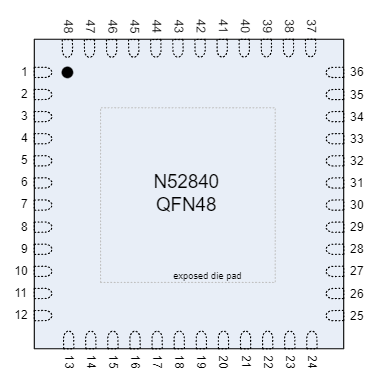
\includegraphics[scale=0.5]{./Figuras/Nota_teorica/Diagrama de pines}
\caption{Diagrama de pines. (Fuente: Imagen tomada de \cite{ST})}
\label{fig:ST_pins}
\end{figure}
A continuación la siguiente tabla muestra las funciones de cada uno de los pines:

\begin{table}[H]
    \centering
    \begin{tabular}{|c|c|c|}
        \hline
        \textbf{Pin} & \textbf{Name} & \textbf{Function} \\
        \hline
        \multicolumn{3}{|c|}{Left side of the chip} \\
        \hline
        1 & DEC1 & Power \\
        2 & P0.00 XL1 & Digital I/O, Analog input \\
        3 & P0.01 XL2 & Digital I/O, Analog input \\
        4 & P0.04 AIN2 & Digital I/O, Analog input \\
        5 & P0.03 AIN3 & Digital I/O, Analog input \\
        6 & P0.07 TRACECLK & Digital I/O, Trace clock \\
        7 & P0.08 & Digital I/O \\
        8 & P1.08 & Digital I/O \\
        9 & P0.09 TRACEDATA0 & Digital I/O, Trace data \\
        10 & P0.10 TRACEDATA1 & Digital I/O, Trace data \\
        11 & P0.11 TRACEDATA2 & Digital I/O, Trace data \\
        12 & VDD & Power \\
        \hline
        \multicolumn{3}{|c|}{Bottom side of the chip} \\
        \hline
        13 & P0.13 & Digital I/O \\
        14 & P0.14 & Digital I/O \\
        15 & P0.17 & Digital I/O \\
        16 & P0.18 nRESET & Digital I/O \\
        17 & VDD & Power \\
        18 & P0.19 & Digital I/O \\
        19 & P0.20 & Digital I/O \\
        20 & P0.21 & Digital I/O \\
        21 & P0.22 & Digital I/O \\
        22 & P0.23 & Digital I/O \\
        23 & P0.24 & Digital I/O \\
        24 & P0.00 TRACEDATA3 & Digital I/O, Trace data \\
        \hline
        \multicolumn{3}{|c|}{Right side of the chip} \\
        \hline
        25 & VDD & Power \\
        26 & SWDIO & Debug \\
        27 & SWDCLK & Debug \\
        28 & NC & - \\
        29 & P0.09 NFC1 & Digital I/O, NFC input \\
        30 & P0.10 NFC2 & Digital I/O, NFC input \\
        31 & ANT & RF \\
        \hline
        \multicolumn{3}{|c|}{-} \\
        \hline
        32 & VSS\_PA & Power \\
        33 & DEC5 & Power \\
        34 & DEC3 & Power \\
        \hline
    \end{tabular}
    \caption{Pinout of the nRF52840 chip}
    \label{tab:nrf52840_pinout}
\end{table}

\begin{table}[H]
    \centering
    \begin{tabular}{|c|c|c|}
        \hline
        \textbf{Pin} & \textbf{Name} & \textbf{Function} \\
        \hline
        35 & XC1 & Analog input \\
        36 & XC2 & Analog input \\
        \hline
        \multicolumn{3}{|c|}{Top side of the chip} \\
        \hline
        37 & VDD & Digital I/O \\
        38 & P1.15 & Digital I/O \\
        39 & P0.03 AIN1 & Digital I/O, Analog input \\
        40 & P0.02 AIN0 & Digital I/O, Analog input \\
        41 & P0.28 AIN4 & Digital I/O, Analog input \\
        42 & P0.29 AIN5 & Digital I/O, Analog input \\
        43 & P0.30 AIN6 & Digital I/O, Analog input \\
        44 & P0.31 AIN7 & Digital I/O, Analog input \\
        45 & VSS & Power \\
        46 & DEC4 & Power \\
        47 & DCC & Power \\
        48 & VDD & Power \\
        \hline
    \end{tabular}
    \caption{Pinout of the nRF52840 chip (Continuation)}
    \label{tab:nrf52840_pinout_cont}
\end{table}


Para más información general del dispositivo, observar el Anexo \ref{an:01_GEN}. Por otro lado, en la Figura \ref{fig:DBLO} puede consultarse el diagrama de bloques del microcontrolador en el cual puede consultarse a alto nivel la conexión interna de este (no incluye el CPU):

\begin{figure}[H]
\centering
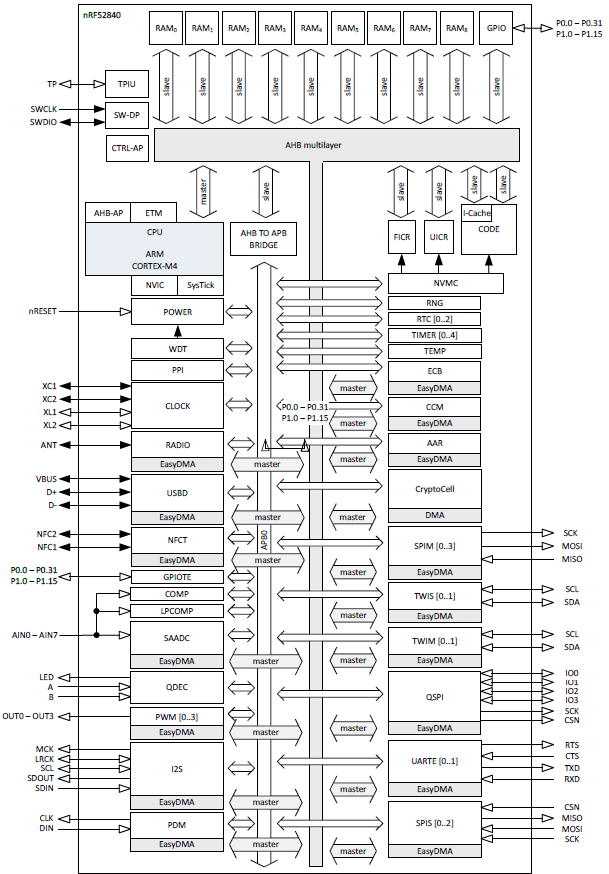
\includegraphics[width=160mm]{./Figuras/Nota_teorica/DIAGRAMA_BLOQUES}
\caption{Diagrama de bloques del nRF52840. (Fuente: Imagen tomada de \cite{ST})}
\label{fig:DBLO}
\end{figure}



\subsubsection{Registros de importancia}
Según la hoja del fabricante \cite{ST}, el mapa de memoria del nRF52840 está dividido en varias regiones, cada una asignada a diferentes tipos de periféricos y funcionalidades. A continuación, se muestran los rangos de direcciones de registros de importancia:

\begin{table}[H]
    \centering
    \scriptsize
    \begin{tabular}{|c|c|c|c|c|}
        \hline
        \textbf{ID} & \textbf{Base address} & \textbf{Peripheral} & \textbf{Instance} & \textbf{Description} \\
        \hline
        0 & 0x40000000 & CLOCK & CLOCK & Clock control \\
        0 & 0x40000000 & POWER & POWER & Power control \\
        0 & 0x50000000 & GPIO & GPIO & General purpose input and output \\
        0 & 0x50000000 & GPIO & P0 & General purpose input and output, port 0 \\
        0 & 0x50000300 & GPIO & P1 & General purpose input and output, port 1 \\
        1 & 0x40001000 & RADIO & RADIO & 2.4 GHz radio \\
        1 & 0x40002000 & UART & UART0 & Universal asynchronous receiver/transmitter \\
        2 & 0x40028000 & UARTE & UARTE0 & Universal asynchronous receiver/transmitter with EasyDMA, unit 0 \\
        3 & 0x40003000 & SPI & SPI0 & SPI master 0 \\
        3 & 0x40003000 & SPIM & SPIM0 & SPI master 0 \\
        3 & 0x40003000 & SPIS & SPIS0 & SPI slave 0 \\
        3 & 0x40003000 & TWI & TWI0 & Two-wire interface master 0 \\
        3 & 0x40003000 & TWIM & TWIM0 & Two-wire interface master 0 \\
        3 & 0x40003000 & TWIS & TWIS0 & Two-wire interface slave 0 \\
        4 & 0x40004000 & SPI & SPI1 & SPI master 1 \\
        4 & 0x40004000 & SPIM & SPIM1 & SPI master 1 \\
        4 & 0x40004000 & SPIS & SPIS1 & SPI slave 1 \\
        4 & 0x40004000 & TWI & TWI1 & Two-wire interface master 1 \\
        4 & 0x40004000 & TWIM & TWIM1 & Two-wire interface master 1 \\
        4 & 0x40004000 & TWIS & TWIS1 & Two-wire interface slave 1 \\
        5 & 0x40005000 & NFCT & NFCT & Near field communication tag \\
        6 & 0x40006000 & GPIOTE & GPIOTE & GPIO tasks and events \\
        7 & 0x40007000 & SAADC & SAADC & Analog to digital converter \\
        8 & 0x40008000 & TIMER & TIMER0 & Timer 0 \\
        9 & 0x40009000 & TIMER & TIMER1 & Timer 1 \\
        10 & 0x4000A000 & TIMER & TIMER2 & Timer 2 \\
        11 & 0x4000B000 & RTC & RTC0 & Real-time counter 0 \\
        12 & 0x4000C000 & TEMP & TEMP & Temperature sensor \\
        13 & 0x4000D000 & RNG & RNG & Random number generator \\
        14 & 0x4000E000 & ECB & ECB & AES electronic code book (ECB) mode block encryption \\
        15 & 0x4000F000 & AAR & AAR & Accelerated address resolver \\
        16 & 0x4000F000 & CCM & CCM & AES counter with CBC-MAC (CCM) mode block encryption \\
        17 & 0x40010000 & WDT & WDT & Watchdog timer \\
        18 & 0x40011000 & RTC & RTC1 & Real-time counter 1 \\
        19 & 0x40012000 & QDEC & QDEC & Quadrature decoder \\
        19 & 0x40013000 & COMP & COMP & General purpose comparator \\
        \hline
    \end{tabular}
    \caption{Rangos direcciones de registros.\cite{ST}}
    \label{tab:nrf52840_peripherals}
\end{table}

\begin{table}[H]
    \centering
    \scriptsize
    \begin{tabular}{|c|c|c|c|c|}
        \hline
        \textbf{ID} & \textbf{Base address} & \textbf{Peripheral} & \textbf{Instance} & \textbf{Description} \\
        \hline
        19 & 0x40013000 & LPCOMP & LPCOMP & Low power comparator \\
        20 & 0x40014000 & EGU & EGU0 & Event generator unit 0 \\
        20 & 0x40014000 & SWI & SWI0 & Software interrupt 0 \\
        21 & 0x40015000 & EGU & EGU1 & Event generator unit 1 \\
        21 & 0x40015000 & SWI & SWI1 & Software interrupt 1 \\
        22 & 0x40016000 & EGU & EGU2 & Event generator unit 2 \\
        22 & 0x40016000 & SWI & SWI2 & Software interrupt 2 \\
        23 & 0x40017000 & EGU & EGU3 & Event generator unit 3 \\
        23 & 0x40017000 & SWI & SWI3 & Software interrupt 3 \\
        24 & 0x40018000 & EGU & EGU4 & Event generator unit 4 \\
        24 & 0x40018000 & SWI & SWI4 & Software interrupt 4 \\
        25 & 0x40019000 & EGU & EGU5 & Event generator unit 5 \\
        25 & 0x40019000 & SWI & SWI5 & Software interrupt 5 \\
        26 & 0x4001A000 & TIMER & TIMER3 & Timer 3 \\
        27 & 0x4001B000 & TIMER & TIMER4 & Timer 4 \\
        28 & 0x4001C000 & PWM & PWM0 & Pulse width modulation unit 0 \\
        29 & 0x4001D000 & PDM & PDM & Pulse Density modulation (digital microphone) interface \\
        30 & 0x4001E000 & ACL & ACL & Access control lists \\
        30 & 0x4001E000 & NVMC & NVMC & Non-volatile memory controller \\
        31 & 0x4001F000 & PPI & PPI & Programmable peripheral interconnect \\
        32 & 0x40020000 & MWU & MWU & Memory watch unit \\
        33 & 0x40021000 & PWM & PWM1 & Pulse width modulation unit 1 \\
        34 & 0x40022000 & PWM & PWM2 & Pulse width modulation unit 2 \\
        35 & 0x40023000 & SPI & SPI2 & SPI master 2 \\
        35 & 0x40023000 & SPIM & SPIM2 & SPI master 2 \\
        35 & 0x40023000 & SPIS & SPIS2 & SPI slave 2 \\
        36 & 0x40024000 & RTC & RTC2 & Real-time counter 2 \\
        37 & 0x40025000 & I2S & I2S & Inter-IC sound interface \\
        38 & 0x40026000 & FPU & FPU & FPU interrupt \\
        39 & 0x40027000 & USBD & USBD & Universal serial bus device \\
        40 & 0x40028000 & UARTE & UARTE1 & Universal asynchronous receiver/transmitter with EasyDMA, unit 1 \\
        41 & 0x40029000 & QSPI & QSPI & External memory interface \\
        42 & 0x5002A000 & CC\_HOST\_RGF & CC\_HOST\_RGF & Host platform interface \\
        43 & 0x5002A000 & CRYPTOCELL & CRYPTOCELL & CryptoCell subsystem control interface \\
        44 & 0x4002D000 & PWM & PWM3 & Pulse width modulation unit 3 \\
        45 & 0x4002F000 & SPIM & SPIM3 & SPI master 3 \\
        \hline
    \end{tabular}
    \caption{Rangos direcciones de registros(Continuación).\cite{ST}}
    \label{tab:nrf52840_peripherals_cont}
\end{table}
\newpage

\subsubsection{Características eléctricas}
A continuación se muestra las especificaciones eléctricas del microcontrolador utilizado:

%%%%%%%%%%%%%%%%%%
\begin{figure}[H]
\centering
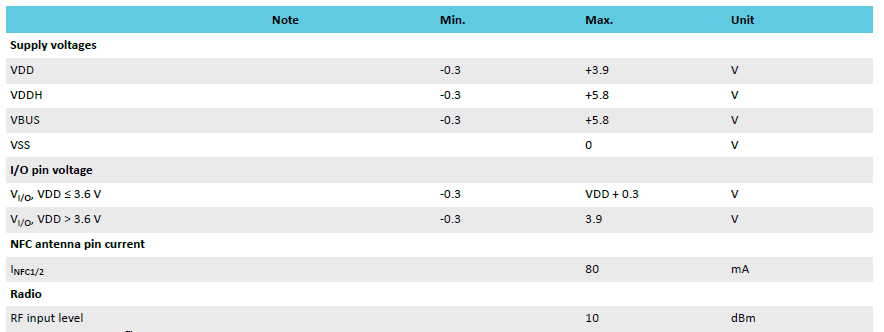
\includegraphics[scale=0.8]{./Figuras/Nota_teorica/ELECTRIC_NRF}
\caption{Características Eléctricas. (Fuente: Imagen tomada de \cite{ST})}
\label{fig:ELEC1}
\end{figure}

%%%%%%%%%%%%%%%%%%
\begin{figure}[H]
\centering
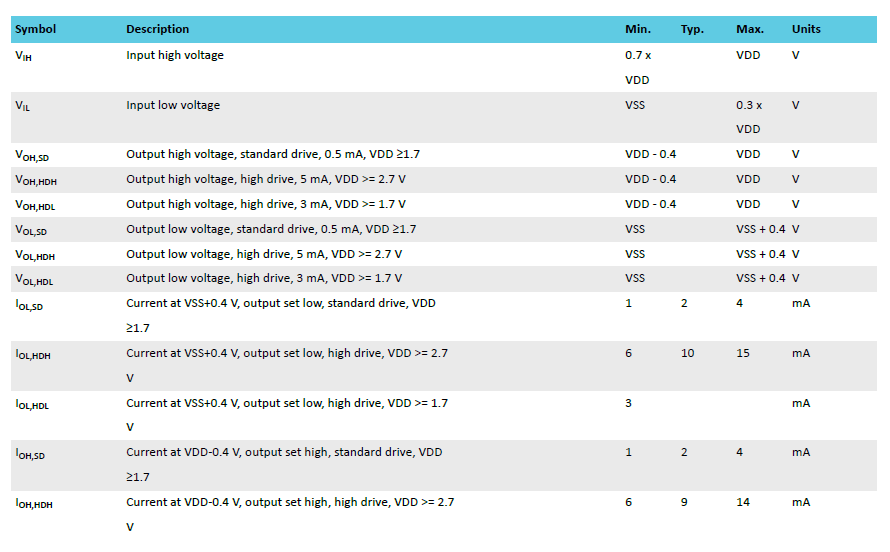
\includegraphics[scale=0.8]{./Figuras/Nota_teorica/GPIO_ELECTRICAL}
\caption{Características electricas GPIO. (Fuente: Imagen tomada de \cite{ST})}
\label{fig:ELEC2}
\end{figure}

\subsection{Arduino Nano 33 BLE sense}
Es una placa de desarrollo de la familia Arduino diseñada para proyectos de Internet de las Cosas (IoT), aplicaciones de aprendizaje automático y sistemas embebidos avanzados. Que utiliza el nRF52840 de Nordic Semiconductor, un microcontrolador ARM® Cortex®-M4 a 64 MHz con Bluetooth. A continuación se muestra la topología de la placa:
\begin{figure}[H]
\centering
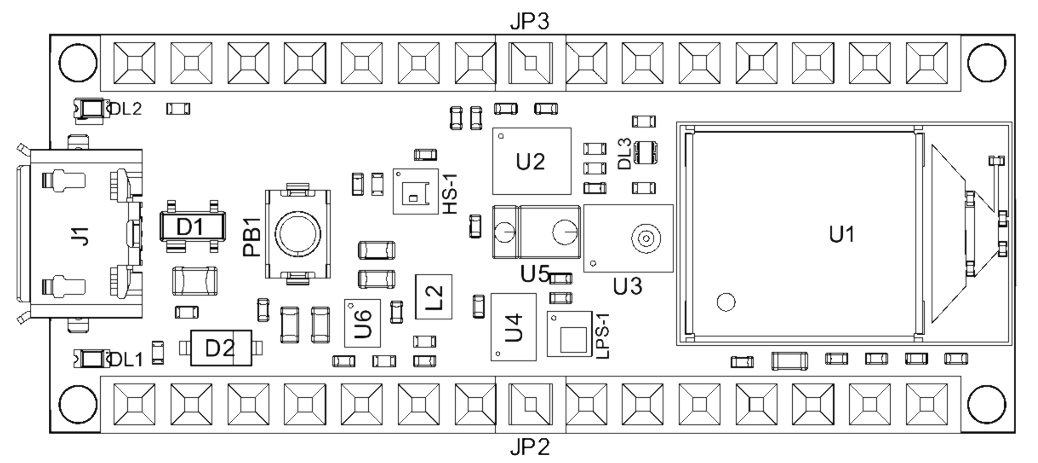
\includegraphics[scale=0.8]{./Figuras/Nota_teorica/Board topology}
\caption{Topología de Nano 33 BLE Sense. (Fuente: Imagen tomada de \cite{arduino_nano33_ble_sense_datasheet})}
\label{fig:nano1}
\end{figure}

A continuación se muestra el diagrama de la placa:
\begin{figure}[H]
\centering
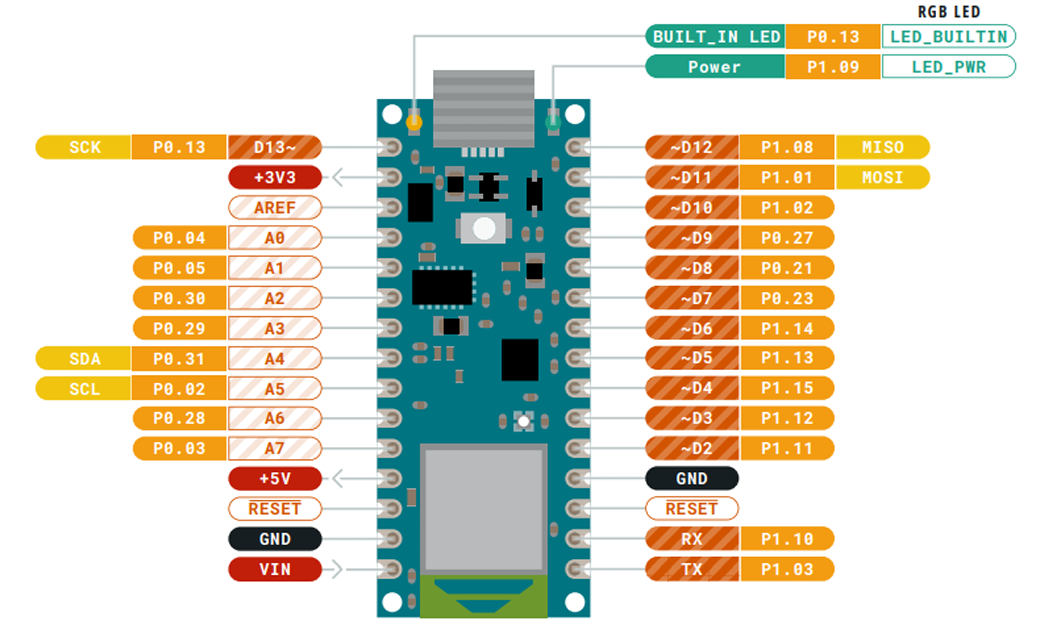
\includegraphics[scale=0.8]{./Figuras/Nota_teorica/PINES_NANO}
\caption{Diagrama pines de Nano 33 BLE Sense. (Fuente: Imagen tomada de \cite{arduino_nano33_ble_sense_datasheet})}
\label{fig:nano2}
\end{figure}
A continuación se muestra una tabla con la descripción de pines de la placa:
\begin{table}[H]
    \centering
    \begin{tabular}{|c|c|c|p{8cm}|}
        \hline
        \textbf{Pin} & \textbf{Function} & \textbf{Type} & \textbf{Description} \\
        \hline
        1 & D13 & Digital & GPIO \\
        \hline
        2 & +3V3 & Power Out & Internally generated power output to external devices \\
        \hline
        3 & AREF & Analog & Analog Reference; can be used as GPIO \\
        \hline
        4 & A0/DAC0 & Analog & ADC in/DAC out; can be used as GPIO \\
        \hline
        5 & A1 & Analog & ADC in; can be used as GPIO \\
        \hline
        6 & A2 & Analog & ADC in; can be used as GPIO \\
        \hline
        7 & A3 & Analog & ADC in; can be used as GPIO \\
        \hline
        8 & A4/SDA & Analog & ADC in; I2C SDA; Can be used as GPIO (1) \\
        \hline
        9 & A5/SCL & Analog & ADC in; I2C SCL; Can be used as GPIO (1) \\
        \hline
        10 & A6 & Analog & ADC in; can be used as GPIO \\
        \hline
        11 & A7 & Analog & ADC in; can be used as GPIO \\
        \hline
        12 & VUSB & Power In/Out & Normally NC; can be connected to VUSB pin of the USB connector by shorting a jumper \\
        \hline
        13 & RST & Digital In & Active low reset input (duplicate of pin 18) \\
        \hline
        14 & GND & Power & Power Ground \\
        \hline
        15 & VIN & Power In & Vin Power input \\
        \hline
        16 & TX & Digital & USART TX; can be used as GPIO \\
        \hline
        17 & RX & Digital & USART RX; can be used as GPIO \\
        \hline
        18 & RST & Digital & Active low reset input (duplicate of pin 13) \\
        \hline
        19 & GND & Power & Power Ground \\
        \hline
        20 & D2 & Digital & GPIO \\
        \hline
        21 & D3/PWM & Digital & GPIO; can be used as PWM \\
        \hline
        22 & D4 & Digital & GPIO \\
        \hline
        23 & D5/PWM & Digital & GPIO; can be used as PWM \\
        \hline
        24 & D6/PWM & Digital & GPIO; can be used as PWM \\
        \hline
        25 & D7 & Digital & GPIO \\
        \hline
        26 & D8 & Digital & GPIO \\
        \hline
        27 & D9/PWM & Digital & GPIO; can be used as PWM \\
        \hline
        28 & D10/PWM & Digital & GPIO; can be used as PWM \\
        \hline
        29 & D11/MOSI & Digital & SPI MOSI; can be used as GPIO \\
        \hline
        30 & D12/MISO & Digital & SPI MISO; can be used as GPIO \\
        \hline
    \end{tabular}
    \caption{Pinout description of Arduino Nano 33 BLE Sense}
    \label{tab:arduino_nano_ble}
\end{table}


\subsection{Módulo de cámara OV7675}

Tal como se describe en \cite{OV}, la cámara Arducam OV7675 proporciona soporte para una resolución de hasta 640x480 píxeles, lo cual la hace ideal para una variedad de proyectos basados en Arduino, incluyendo sistemas de automatización del hogar y dispositivos inteligentes de monitoreo que necesitan entrada visual precisa. La OV7675 ofrece una interfaz fácil de usar y es capaz de generar salida en formatos RAW, YUV y RGB. Sus especificaciones incluyen un tamaño de píxel de 2.5 $\mu$m, una relación señal/ruido de 38 dB y un rango de temperatura operativa amplio, desde -30°C hasta 70°C. Con un tamaño compacto de placa de 30.5mm x 30.5mm, esta cámara destaca por su versatilidad y calidad de imagen en diversas condiciones ambientales. En la Figura \ref{fig:OV7675} puede observarse el módulo de cámara utilizado para este proyecto: 

\begin{figure}[H]
\centering
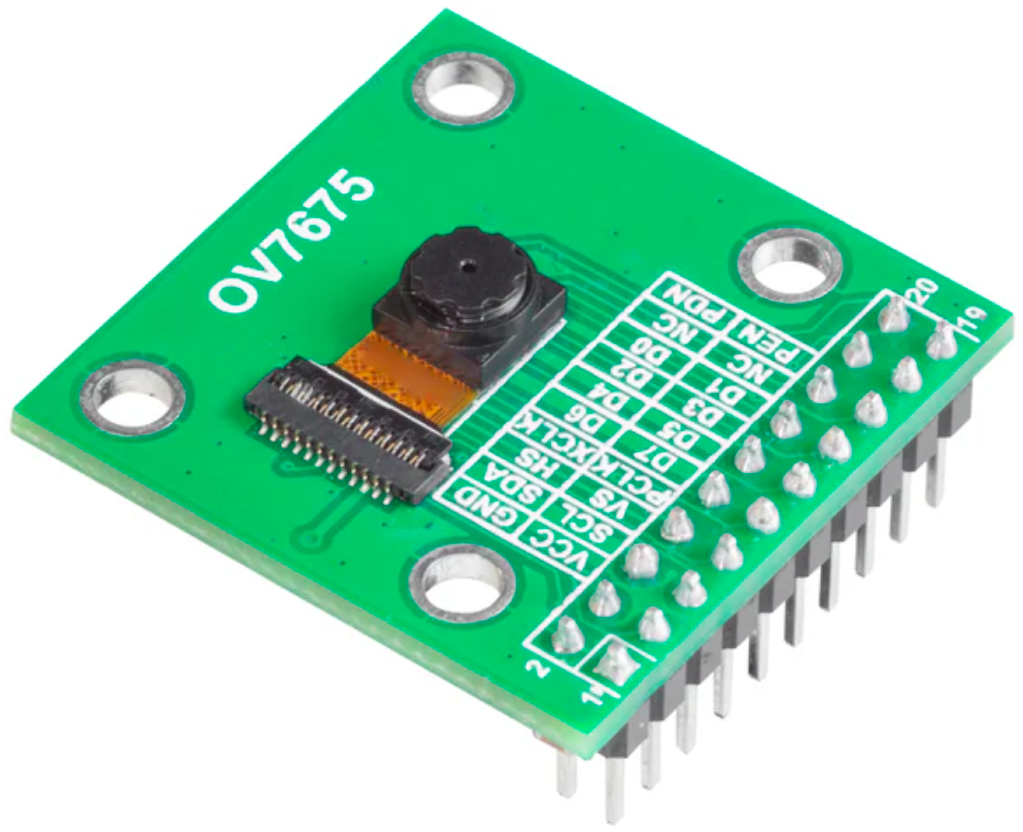
\includegraphics[width=80mm]{./Figuras/Nota_teorica/OV7675}
\caption{Módulo de cámara OV7675 utilizado en el laboratorio. (Fuente: Imagen tomada de \cite{OV}).} 
\label{fig:OV7675}
\end{figure}

\subsection{Librerías de importancia}

A continuación se detallan las librerías que fueron utilizadas en el laboratorio:
\subsubsection{Arduino\_OV767X}
La librería Arduino\_OV767X proporciona una interfaz para utilizar la cámara OV7670/OV7675 con placas Arduino. Esta librería simplifica la captura y procesamiento de imágenes directamente desde la cámara, permitiendo a los desarrolladores incorporar funcionalidades de visión por computadora en sus proyectos de Arduino. Entre sus funcionalidades, se incluyen la configuración de la resolución de imagen, la captura de imágenes en formato RGB y la gestión de buffers de imagen.
\subsubsection{stdint.h}
La librería stdint.h es una parte estándar de la biblioteca de C y C++ que define tipos de datos enteros con tamaños específicos. Esta librería es fundamental en programación de sistemas embebidos, donde es crucial manejar tipos de datos con tamaños bien definidos para garantizar el uso eficiente de la memoria y el rendimiento del sistema.
\subsubsection{stdlib.h}
 La librería stdlib.h es una parte estándar de la biblioteca de C que proporciona funciones para la gestión de memoria, generación de números aleatorios, conversión de tipos y otros utilitarios generales. Es una librería fundamental en la programación en C y C++, proporcionando herramientas esenciales para el desarrollo de aplicaciones.
 
\subsection{Machine Learning}
\textit{Machine Learning} o Aprendizaje de maquina, es un subcampo de la inteligencia artificial. Este ayuda a los ordenadores a aprender y actuar como seres humanos mediante la ayuda de algoritmos y datos. Dado un conjunto de datos, un algoritmo de aprendizaje maquina aprende diferentes propiedades de los datos e infiera que propiedades de los datos se pueden presentar en el futuro. A diferencia de los sistemas tradicionales que siguen instrucciones preprogramadas, los sistemas de Machine Learning mejoran su rendimiento a medida que se les proporciona más datos \cite{jimenez2021introduccion}. Algunos conceptos clave para desenvolverse en el mundo de \textit{machine learning} son:
\begin{itemize}
    \item \textbf{Datos de entrenamiento:} Conforman los datos que se incorporan al algoritmo de aprendizaje maquina para entrenar el modelo.
    \item \textbf{Datos de prueba:} Constituyen los datos utilizados para validar la presición del modelo.
    \item \textbf{Sobreentrenamiento:} Ocurre cuando un modelo aprende los datos de entrenamiento de manera tan precisa o exacta que pierde la capacidad de generalizar.
    \item \textbf{Subentrenamiento:} Ocurre cuando el modelo no a aprendido lo suficiente la estructura de los datos.
    \item \textbf{Aprendizaje Supervisado:} El modelo se entrena con datos etiquetados, lo que significa que cada dato de entrenamiento está asociado a una etiqueta o resultado deseado.
    \item \textbf{Aprendizaje No Supervisado:} El modelo se entrena con datos que no están etiquetados. El objetivo es encontrar patrones o estructuras en los datos.
\end{itemize}

\subsection{TinyML}
Según se describe en \cite{TML}, TinyML es un campo especializado centrado en desplegar modelos de aprendizaje automático en dispositivos pequeños y con recursos limitados, como microcontroladores y sensores. Esta tecnología es fundamental para habilitar el concepto de \textit{edge computing}, donde los datos pueden procesarse localmente en los dispositivos sin necesidad de enviarlos a un servidor centralizado o a la nube. Al aprovechar algoritmos ligeros y técnicas de optimización de modelos, TinyML asegura que las capacidades de aprendizaje automático puedan operar eficientemente dentro de los recursos computacionales limitados y las restricciones de energía de estos dispositivos.

Una de las principales ventajas de TinyML es su capacidad para reducir la latencia y permitir el procesamiento en tiempo real. Al realizar el análisis de datos localmente, las aplicaciones de TinyML pueden lograr tiempos de respuesta más rápidos en comparación con las soluciones tradicionales basadas en la nube, lo cual es crucial para aplicaciones que requieren decisiones inmediatas. Además, TinyML mejora la eficiencia energética al minimizar la carga computacional en los dispositivos. En cuanto a las aplicaciones, TinyML tiene una amplia gama de usos. Puede ser utilizado en el sector de la salud para monitoreo continuo y diagnóstico y en vehículos autónomos para mejorar las capacidades de navegación y toma de decisiones. 

\subsection{TensorFlow Lite}
TensorFlow Lite es un conjunto de herramientas diseñado para el aprendizaje automático en dispositivos, optimizado para ejecutarse en dispositivos celulares, empotrados y \textit{edge} \cite{TFL}. Ofrece soporte multiplataforma (Android, iOS, Linux empotrado, microcontroladores) y es compatible con varios lenguajes (Java, Swift, Objective-C, C++, Python). Sus características clave incluyen alta eficiencia en términos de latencia, privacidad (los datos no salen del dispositivo), conectividad (no requiere conexión a internet), tamaño reducido de modelos y consumo eficiente de energía. Facilita la generación de modelos mediante la conversión de modelos existentes o la creación de nuevos, y permite la ejecución de inferencias utilizando APIs adaptadas para modelos con o sin metadatos.

\subsection{Edge Impulse}
Es una plataforma especializada en el desarrollo y despliegue de modelos de Machine Learning (ML) y de inteligencia artificial (IA) en dispositivos con capacidades limitadas, comúnmente conocidos como dispositivos edge. Esta plataforma facilita la creación, el entrenamiento, la optimización y el despliegue de modelos ML en dispositivos de bajo consumo, tales como microcontroladores y sistemas integrados, sin necesidad de tener una profunda experiencia en ML o IA. Esta plataforma se caracteriza por tener una interfaz amigable con el usuario, que proporciona guías para facilitar el proceso de creación de modelos. Además es compatible con una amplia gama de hardware incluyendo microcontroladores de distintos fabricantes como Arduino, STMicroelectronics, Nordic Semiconductor entre otros. Una característica importante de Edge impulse es que permite el entrenamiento de modelos en la nube, aprovechando recursos computacionales potentes sin necesidad de hardware especializado por parte del usuario \cite{Impulse_2020}.

\subsection{Configuración y parámetros de la red neuronal en Edge Impulse}  
Una vez que el proceso de diseño de las partes del impulso fue concluido, debe procederse con el \textit{Transfer Learning}, para el cual deben ser seleccionados un grupo de parámetros. Una breve explicación de los parámetros que pueden ser modificados para ajustar el entrenamiento del modelo pueden observarse a continuación, según se explica en \cite{EIP}: 

\begin{itemize}
    \item \textit{\textbf{Number of training cycles}}: corresponde a la cantidad de veces que el algoritmo de entrenamiento realiza un paso completo a través de todos los datos de entrenamiento con retropropagación y actualiza los parámetros del modelo mientras avanza.

    \item \textit{\textbf{Learning rate}}: maneja cuánto se actualizan los parámetros internos del modelo durante cada paso del proceso de entrenamiento. También se puede entender como la velocidad a la que la red neuronal aprenderá. Si la red se sobre-ajusta rápidamente, se puede reducir la tasa de aprendizaje.

    \item \textit{\textbf{Data augmentation}}: habilita la transformación aleatoria de los datos durante el entrenamiento. Permite ejecutar más ciclos de entrenamiento sin sobre-ajustarlo, lo que puede mejorar la precisión.

    \item \textit{\textbf{Validation set size}}: es el porcentaje del conjunto de entrenamiento reservado para validación, siendo un buen valor por defecto el 20\%.

    \item \textit{\textbf{Split train/validation set on metadata key}}: permite prevenir la fuga de datos entre conjuntos de entrenamiento y validación agrupando datos mediante metadatos. Se debe dejar vacío para deshabilitar esta opción.

    \item \textit{\textbf{Batch size}}: define el tamaño del \textit{batch} (se refiere al n[umero de ejemplos de entrenamiento utilizados en cada iteración). Si no se establece, se utilizará el valor predeterminado. El entrenamiento podría fallar si el tamaño del \textit{batch} es demasiado grande. 

    \item \textit{\textbf{Auto-weight classes}}: habilita que durante el entrenamiento se preste más atención a las muestras de clases menos representadas. Puede ayudar a que el modelo sea más robusto contra el sobre-ajuste si se dispone de pocos datos para algunas clases.

    \item \textit{\textbf{Profile int8 model}}: analizar el modelos cuantizados puede llevar mucho tiempo en conjuntos de datos grandes. Deshabilitar esta opción para omitir el perfilado.
\end{itemize}

Otra sección de importancia es la de selección de la \textbf{arquitectura de la red neuronal}. Tal como se explica en \cite{EIP}, la arquitectura de red neuronal toma como entradas las características extraídas, y pasa las características a cada capa de su arquitectura. En el caso de la clasificación, la última capa utilizada es una capa \textit{softmax} (toma las puntuaciones de salida brutas de la capa anterior y las transforma en probabilidades sumadas da como resultado 1). Es esta última capa la que da la probabilidad de pertenecer a una de las clases predefinidas.

\subsection{Lista de componentes y precios}

Para el presente laboratorio sólo fue necesario el \textit{Tiny Machine Learning Kit} de Arduino, el cual puede obtener a través de la tienda de Arduino por \$60.00 (consultar \url{https://store-usa.arduino.cc/products/arduino-tiny-machine-learning-kit?selectedStore=us}). Para realizar este proyecto son necesarios ₡31,403.70, según el valor del dólar al momento de escribir el presente informe. El contenido de este kit puede observarse en la Tabla \ref{table:Equipo} a continuación:  

\begin{table}[H]
\caption{Lista de componentes.}
\begin{center}
\begin{tabular}{c|c}
\hline
\textbf{Componente}&\textbf{Cantidad}\\
\hline
Arduino Nano 33 BLE Sense board & 1 \\
OV7675 Camera & 1 \\
Arduino Tiny Machine Learning Shield & 1 \\
USB A to Micro USB Cable & 1 \\
\hline
\end{tabular} \label{table:Equipo}
\end{center}
\end{table}